%license:BSD-3-Clause
%copyright-holders:Michele Maione
%============================================================
%
%	Cloud gaming platform for arcade games
%
%============================================================
\chapter{Tecnologie}

Lorem ipsum dolor sit amet, consectetur adipiscing elit, sed do eiusmod tempor incididunt ut labore et dolore magna aliqua. Ut enim ad minim veniam, quis nostrud exercitation ullamco laboris nisi ut aliquip ex ea commodo consequat. Duis aute irure dolor in reprehenderit in voluptate velit esse cillum dolore eu fugiat nulla pariatur. Excepteur sint occaecat cupidatat non proident, sunt in culpa qui officia deserunt mollit anim id est laborum.

\section{MPEG}
Lorem ipsum dolor sit amet, consectetur adipiscing elit, sed do eiusmod tempor incididunt ut labore et dolore magna aliqua. Ut enim ad minim veniam, quis nostrud exercitation ullamco laboris nisi ut aliquip ex ea commodo consequat. Duis aute irure dolor in reprehenderit in voluptate velit esse cillum dolore eu fugiat nulla pariatur. Excepteur sint occaecat cupidatat non proident, sunt in culpa qui officia deserunt mollit anim id est laborum.

\subsection{Compression}
Lorem ipsum dolor sit amet, consectetur adipiscing elit, sed do eiusmod tempor incididunt ut labore et dolore magna aliqua. Ut enim ad minim veniam, quis nostrud exercitation ullamco laboris nisi ut aliquip ex ea commodo consequat. Duis aute irure dolor in reprehenderit in voluptate velit esse cillum dolore eu fugiat nulla pariatur. Excepteur sint occaecat cupidatat non proident, sunt in culpa qui officia deserunt mollit anim id est laborum.

\subsection{Video}
Lorem ipsum dolor sit amet, consectetur adipiscing elit, sed do eiusmod tempor incididunt ut labore et dolore magna aliqua. Ut enim ad minim veniam, quis nostrud exercitation ullamco laboris nisi ut aliquip ex ea commodo consequat. Duis aute irure dolor in reprehenderit in voluptate velit esse cillum dolore eu fugiat nulla pariatur. Excepteur sint occaecat cupidatat non proident, sunt in culpa qui officia deserunt mollit anim id est laborum.

\subsection{Audio}
Lorem ipsum dolor sit amet, consectetur adipiscing elit, sed do eiusmod tempor incididunt ut labore et dolore magna aliqua. Ut enim ad minim veniam, quis nostrud exercitation ullamco laboris nisi ut aliquip ex ea commodo consequat. Duis aute irure dolor in reprehenderit in voluptate velit esse cillum dolore eu fugiat nulla pariatur. Excepteur sint occaecat cupidatat non proident, sunt in culpa qui officia deserunt mollit anim id est laborum.

\subsection{Trasmission}
Lorem ipsum dolor sit amet, consectetur adipiscing elit, sed do eiusmod tempor incididunt ut labore et dolore magna aliqua. Ut enim ad minim veniam, quis nostrud exercitation ullamco laboris nisi ut aliquip ex ea commodo consequat. Duis aute irure dolor in reprehenderit in voluptate velit esse cillum dolore eu fugiat nulla pariatur. Excepteur sint occaecat cupidatat non proident, sunt in culpa qui officia deserunt mollit anim id est laborum.



\section{FFmpeg}
Lorem ipsum dolor sit amet, consectetur adipiscing elit, sed do eiusmod tempor incididunt ut labore et dolore magna aliqua. Ut enim ad minim veniam, quis nostrud exercitation ullamco laboris nisi ut aliquip ex ea commodo consequat. Duis aute irure dolor in reprehenderit in voluptate velit esse cillum dolore eu fugiat nulla pariatur. Excepteur sint occaecat cupidatat non proident, sunt in culpa qui officia deserunt mollit anim id est laborum\cite{FFmpeg_Documentation}.

\subsection{Libs.}
Lorem ipsum dolor sit amet, consectetur adipiscing elit, sed do eiusmod tempor incididunt ut labore et dolore magna aliqua. Ut enim ad minim veniam, quis nostrud exercitation ullamco laboris nisi ut aliquip ex ea commodo consequat. Duis aute irure dolor in reprehenderit in voluptate velit esse cillum dolore eu fugiat nulla pariatur. Excepteur sint occaecat cupidatat non proident, sunt in culpa qui officia deserunt mollit anim id est laborum.



\section{Simple DirectMedia Layer (SDL)}
SDL is a library that provides low level access to audio, keyboard, mouse, joystick, 3D hardware, and 2D framebuffer across multiple platforms, also mobile. SDL it is built on top of the video display APIs of the O.S., a 3D rendering library and a library that interface to sound card\cite{SDL_Wiki}.

\begin{figure}[H]
	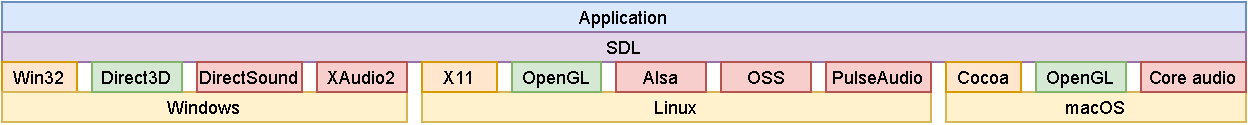
\includegraphics[width=\linewidth]{immagini/sdl}
	\caption{Abstraction layers of several SDL platforms}
	\label{fig:sdl}
\end{figure}

\subsection{Video}
The MAME is able to emulate 3D games but since a physical monitor is being emulated, what is sent to the various graphics libraries is a set of primitives and textures to be drawn, and for this reason the drawing is always carried out in 2D.

\begin{figure}[H]
	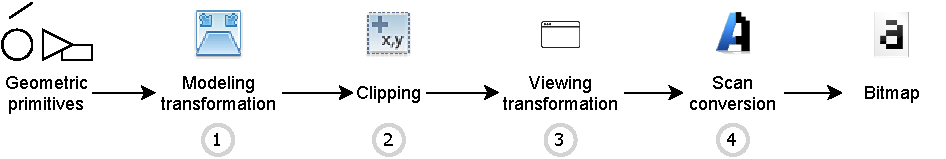
\includegraphics[width=\linewidth]{immagini/rendering_pipeline}
	\caption{2D rendering pipeline}
	\label{fig:rendering_pipeline}
\end{figure}

When the window is initialized an SDL 2D rendering context for the window is created through the function \textit{CreateRenderer}. For each emulated machine frame there is a draw phase using \textit{SetRenderDrawColor}, \textit{RenderFillRect} and \textit{RenderDrawLine}. In the end the function \textit{RenderPresent} is used to show the frame on the window.

In section \ref{SDL_renderer} other functions, used to modify this standard behaviour descripted above, are introduced.


\subsection{Audio}
Lorem ipsum dolor sit amet, consectetur adipiscing elit, sed do eiusmod tempor incididunt ut labore et dolore magna aliqua. Ut enim ad minim veniam, quis nostrud exercitation ullamco laboris nisi ut aliquip ex ea commodo consequat. Duis aute irure dolor in reprehenderit in voluptate velit esse cillum dolore eu fugiat nulla pariatur. Excepteur sint occaecat cupidatat non proident, sunt in culpa qui officia deserunt mollit anim id est laborum.



\section{Web APIs}
Web APIs are a set of APIs and interfaces that comprise the Web's powerful scriptability. Following those used in this project\cite{Web_APIs}.

\subsection{WebSocket}
WebSocket is a computer communications protocol providing full-duplex communication channels over a single TCP connection. It is compatible with HTTP because the WebSocket handshake uses the HTTP upgrade header to switch from the HTTP to the WebSocket protocol. It is natively supported by all browsers and its use is similar to normal sockets on both client and server sides. For these reasons it is the most used generic communication protocol on the web\cite{WebSocket_Web_APIs}.

\subsection{Canvas API}
The Canvas API provides a means for drawing graphics via JavaScript, is largely focuses on 2D graphics but when used by WebGL API can draws hardware-accelerated 2D and 3D graphics. It is fully supported by all browsers\cite{Canvas_API}.

\subsection{WebGL API}
WebGL is a JavaScript API, designed and maintained by the non-profit Khronos Group, for rendering interactive 2D and 3D graphics allowing GPU-accelerated usage of physics and image processing and effects. WebGL 1.0 is supported on all browsers, while WebGL 2.0 is being tested on Safari\cite{WebGL}.



\section{JavaScript libraries}
For the front-end, opensource JavaScript libraries were used for the input management and for decoding the movie.

\subsection{JSMpeg}
JSMpeg is a JavaScript library that consists of an MPEG-TS demuxer, MPEG1 video and MP2 audio decoders, WebGL and Canvas2D renderers and WebAudio sound output. JSMpeg can load static videos via Ajax and allows low latency streaming ($\sim$50ms) via WebSockets, it is released under the MIT License\cite{JSMpeg}.

\subsection{Keypress}
Keypress is a keyboard input capturing JavaScript utility focused on input for games, released under the Apache License 2.0. It is used to handle keyboard input in the front-end\cite{Keypress}.

\subsection{GameController.js}
GameController.js is a library that uses JavaScript and the standard Gamepad API, it is released under the MIT License. In the front-end it is used to manage gamepads, to allow couch multiplayer\cite{gameController_js}.